\documentclass{acm_proc_article-sp}
\usepackage[lined,boxed,commentsnumbered]{algorithm2e}
\usepackage{amsmath}
\usepackage{graphicx}
\usepackage{url}
\usepackage{multirow}

\begin{document}

\title{PushUp: An event-based http Long-polling Server}

\numberofauthors{2}
\author{
% 1st. author
\alignauthor
Kai Liu \\
       \affaddr{Very Large Information System}\\
       \affaddr{Carnegie Mellon University}\\
       \email{hfevers@gmail.com}
% 2nd. author
\alignauthor
Yilun Cui \\
       \affaddr{Very Large Information System}\\
       \affaddr{Carnegie Mellon University}\\
       \email{yiluncui@gmail.com}
}

\maketitle

\begin{abstract} 

The ``long-polling" is a server push technology that makes the delivery of the 
latest updates from server to clients more ``instant". With long polling, 
when a client requests updated information from the server, the server
will keep the request connection open if there is no available information yet. 
The server sends the complete response to the client only when the interested
information becomes available or after a suitable timeout.

However this solution may require the server to hold large number of open 
connections for in the server side. To efficiently manage these connections
and reduce the complexity of web development, we propose an event-driven, 
dedicated long-polling server to provide efficient and scalable long polling
services for the web servers. To prove its efficiency, we compare
the performance of PushUp server and several other server-side event 
notification methods. The experimental results confirms the PushUp server's 
excellent capacity in serving large number of concurrent connections with 
much less resource.

\end{abstract}

\section {Introduction\\}
Traditionally, the web server is a classical example of the request/response 
model, where the clients can retrieve the resource from the server but the 
server cannot push the data to the client actively. 

However, with the increasing popularity of Ajax\cite{Ajax} technologies, there 
are many scenarios where servers would like to actively notify the clients the 
latest updates. For example, the new messages in chat room, latest tweets in 
twitter, etc.

To overcome the limitation of request/response model, many approaches has been 
proposed to build more responsive sites. For example:

\begin{itemize}
\item Client Pull: the client sends update requests periodically to pull the
updates from server. This method is very easy to implement because 
it is stateless and the web server doesn't need to put much effort to modify 
its architecture. However, client pull will generate lots of http requests.
The work flow of client pull is illustrated in Figure \ref{fig:client_pull}.

\item Plugins: since the HTTP itself doesn't provide any mechanism for server 
push, plugins, such as the Flash, Silverlight, Javelet, etc, can be used as an 
extension of the HTTP by providing more flexible client/server communication 
mechanisms. However plugins is non-standard and requires users' extra effort to 
install and configure them.
\end{itemize}

Given those drawbacks, we focus on the another solution: long polling
\cite{LongPolling}. The work flow of long polling can be described in Figure
\ref{fig:long_polling}. When a client ``asks for"(polls) an update by sending 
an HTTP request to the server, if the no information is yet available, the 
server will not terminate the connection immediately; Instead, the server 
will keep the connection open for a period of time until (1) the information 
become available (2) after a suitable timeout($50$ seconds is a common choice).

The benefit to long-polling is that there is less back-and-forth between the 
client and server. The server is in control of the timing, so updates to the
browser can be made within milliseconds. This makes it ideal for some highly
interactive web applications.

\begin{figure}[htb!]
\centering
    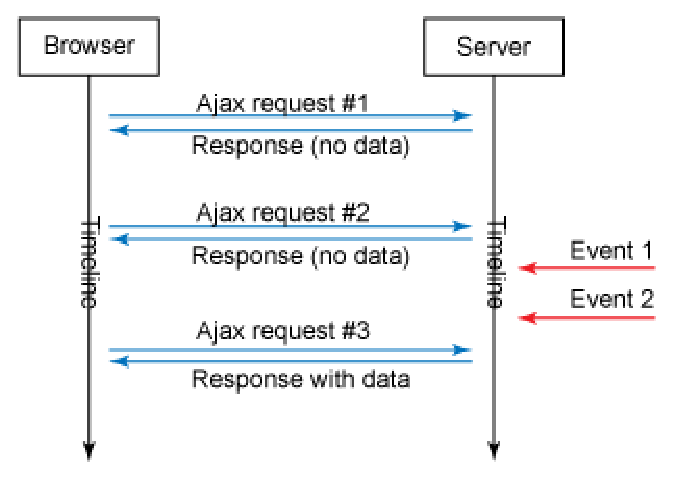
\includegraphics[scale=0.70]{figures/client_pull.eps}
    \caption{Client Pull Work Flow}
    \label{fig:client_pull}
\end{figure}

\begin{figure}[htb!]
    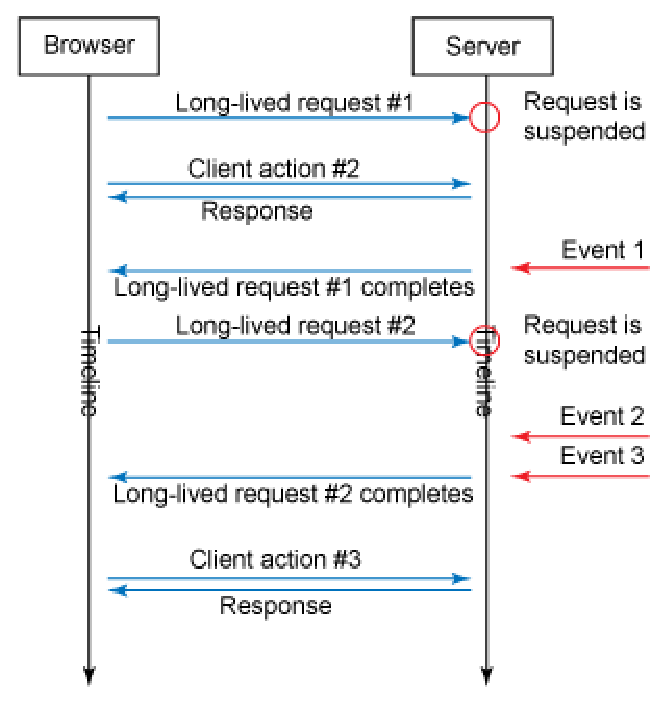
\includegraphics[scale=0.70]{figures/long_polling.eps}
    \caption{Long Polling Work Flow}
    \label{fig:long_polling}
\end{figure}

The down-side of long polling is that the server may have to deal with large
number of active connections between the clients and the servers. For example,
if you have one million users and, 10\% of them will be online. In this case,
the server should be able to hold at least 100,000 concurrent connections.

To address these problems, we present the event-based\cite{UnixBook}, scalable
long polling server PushUp to provide dedicated long polling services for 
different web applications with less resource cost.

As illustrated in Figure \ref{fig:sim_pushup}, the PushUp server lies in 
between of clients and web servers. It has two main responsibilities:
\begin{figure}[htb!]
\centering
    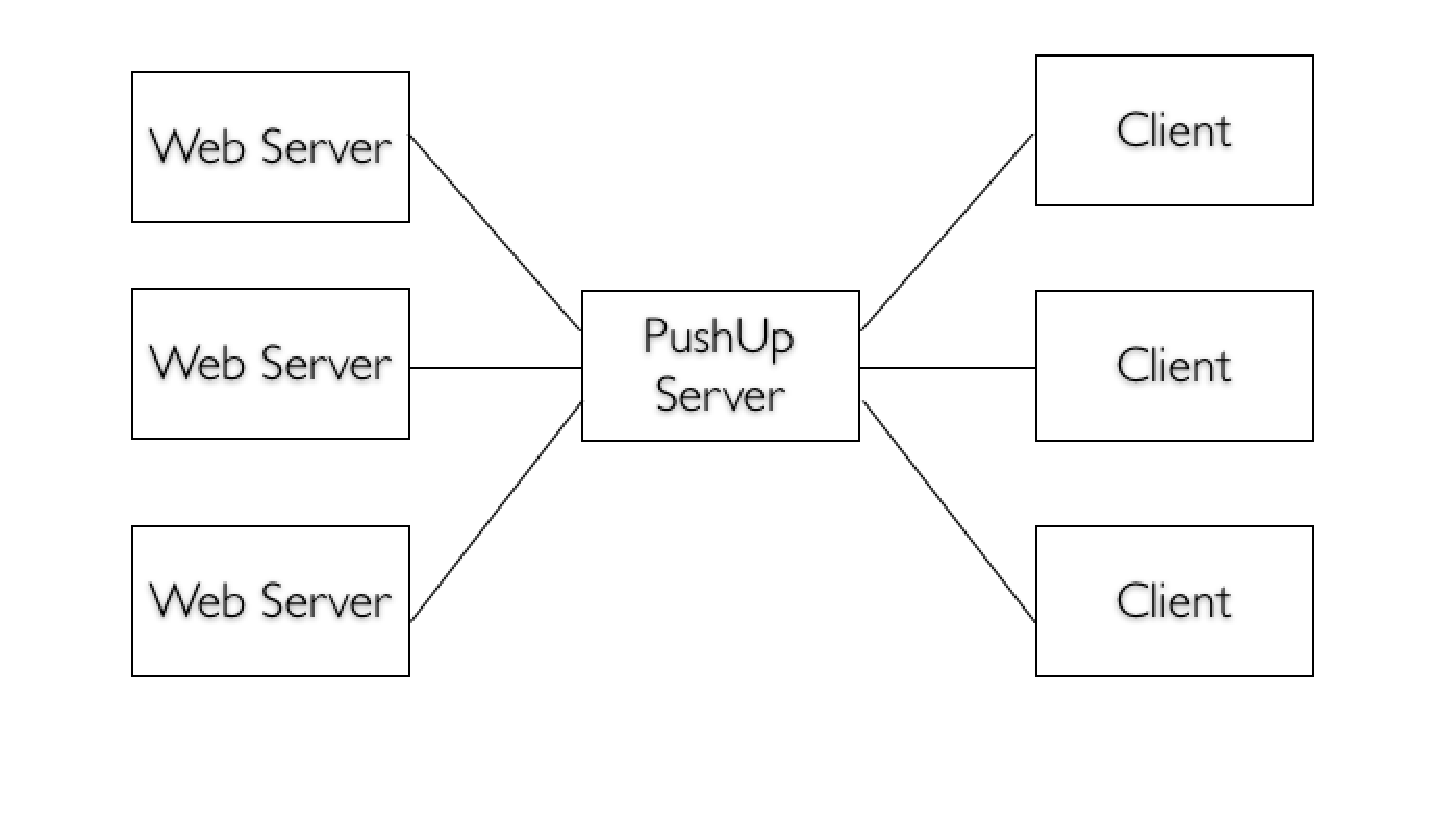
\includegraphics[scale=0.40]{figures/sim_pushup.eps}
    \caption{Simplified Architecture of the PushUp}
    \label{fig:sim_pushup}
\end{figure}

\begin {itemize}
\item {\bf An event-based message queue}\cite{PubSub} to provide the long 
polling services. It keeps the active connections with very low overhead.
The core to this component is an event-based message queue provides
publication interface for the web servers and the subscription interface
for the clients.
\item {\bf An event-based reverse proxy}\cite{ReverseProxy} that retrieves 
resources on behalf of a client from one or more servers.
\end {itemize}

The message queue and reverse proxy of PushUp server forms an intermediary
between browsers and web servers. When a client request arrives the PushUp
will forward non-update-polling to the backend web servers and the long 
polling requests to the message queues. Doing this allows both clients and
web servers work with minimal awareness of PushUp Server. 

\section {System Overview}
\subsection{Problem with the existing designs\\}

\subsection{Design Goals and Rationale\\}

\begin{itemize}
\item {\bf Scalability}  
    As the long polling technologies requires the server to keep the polliing request active for a period of time,
    large number of concurrent clients will generate lots of active connections. One of our goal is to minimize the 
    cost of maintaining these active connections, which could in turn enhance the system's scalability.
     
    Scalability is the main issue in a Push model. Web servers usually create a thread per
    client (connection). However, an HTTP based push will have an
    outstanding request waiting on the server which will be used to send a response to the
    client the instant an asynchronous event occurs. 
    
    However, for the http-based polling request, a large portion of the time will spent in waiting for new events, which
    makes the traditonal multi-thread model inefficient. Better technologies are needed 

\item {\bf Transparancy} TODO: many backend are implement in multi-thread model, so ... be able to have the long polling service with minimal effort (with little modification of the original service).

\item {\bf Low latency} TODO: overhead is inevitable, how to minimize it?

\item {\bf Generality} TODO: can be used in many scenarios.

\end{itemize}

\subsection{System Overview\\}

TODO: a figure to illustrate the main idea.

TODO: Overall description of such design. and how it matches the rationale mentioned above.


\subsection{Reverse Proxy\\}

Why reverse proxy

How it works. Briefly

\subsection{Message Queue\\}

Why Message Queue, 

How it works, briefly



\section {Design and Implementation\\}

\subsection{Reactor Model\\}
The PushUp server runs atop of the Twisted framework\cite{Twisted}, an 
event driven framework that implements the ``reactor" style event loop.

The reactor patterns is an event processing pattern for handling concurrent
service requests. It demultiplexes these requests to associated event
handlers(implemented as the callback). The event handler performs
the actual read or write synchronously.

In our project the reactor manages event loops (one Reactor 
can start several event loops) and runs in a single thread. The
Twisted's event loop has well encapsulated the OSes' underlying 
event notification mechanism (for example, kqueue() in FreeBSD 
and epoll() in Linux).
During execution, the event loop manages the details regarding to
event handler registrations, the activations of event handlers, etc.

The advantage of the reactor pattern is the complete separation of the 
application specific code from reactor's implementations. That is to
say, the application components can be easily divided into reusable 
modules. Also, running the reactor in a single thread significantly
reduce the concurrency controls since no other threads will contend 
the system resource instantaneously.

Figure \ref{fig:mainloop} demonstrates the how the execution switches
between the event loops and user code. Figure \ref{fig:eventloop_flow} 
further illustrates the detailed work flow with sequence diagram.

As we can see from these figures, one of the caveats of in 
event-driven development is that all the event handlers should 
be carefully designed in order to make sure its execution time 
will not take a long time; otherwise other pending actions will
be blocked on this operation.

\begin{figure}[htb!]
    \centering%
    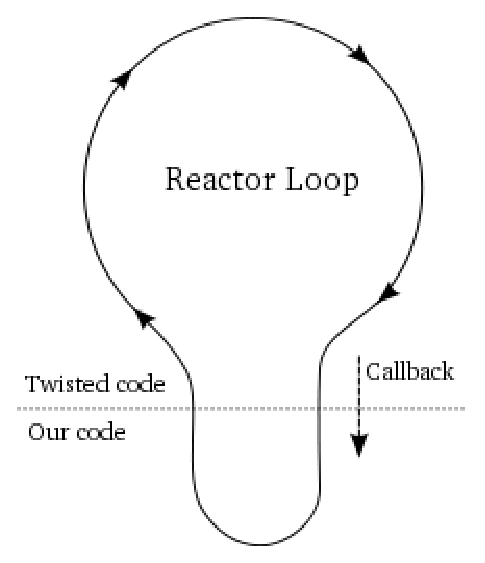
\includegraphics[scale=0.75]{figures/mainloop.eps}
    \caption{Work flow of Twisted Reactor Model}
    \label{fig:mainloop}
\end{figure}
\begin{figure}[htb!]
    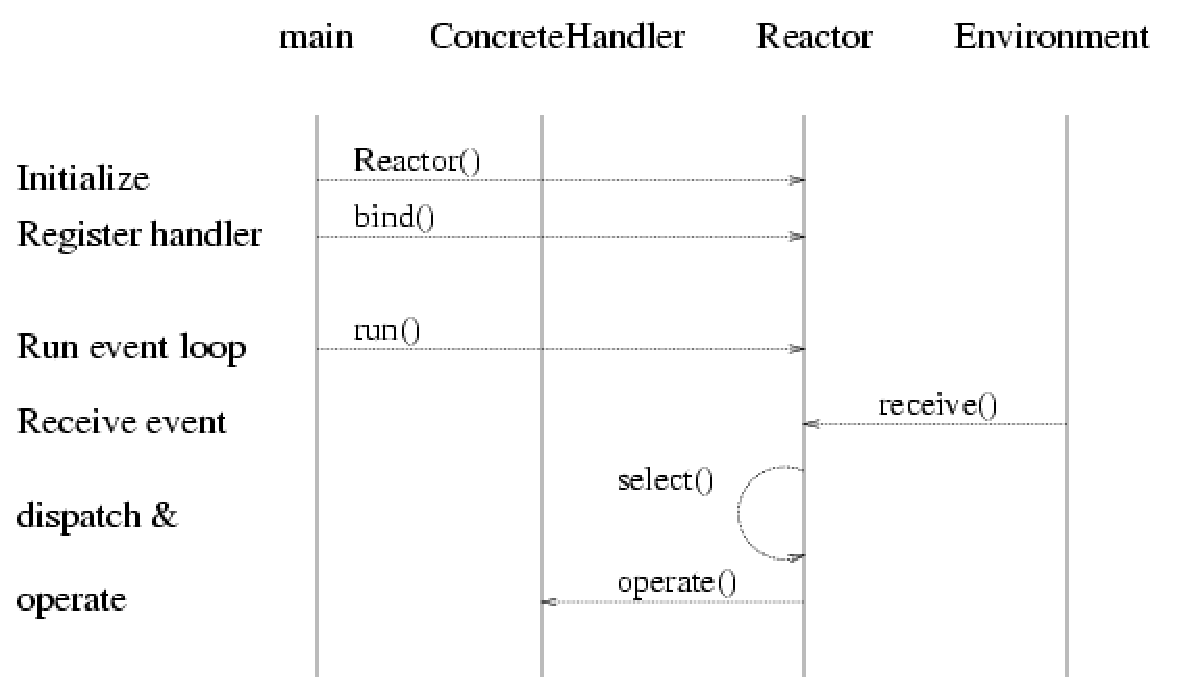
\includegraphics[scale=0.45]{figures/eventloop_flow.eps}
    \caption{The Sequence Diagram of the Event Loop}
    \label{fig:eventloop_flow}
\end{figure}


\subsection{Channels\\}

A ``channel" represents message stream of a certain type. For example, a
channel may be used to represent the feed of a specific user's tweets in
twitter, or the articles of a blog. The channel is the building block of 
PushUp's message queue.

The channel has two major responsibilities: manages the subscription and
incoming messages in this channel.

A complete subscription includes the following information:

\begin{itemize}
    \item {\bf Timeout(required)}: the channel will keep the subscription 
        connection open only for a certain timespan. If nothing happens 
        during this period, the
        subscription request will be terminated and removed from the active 
        subscription list by the channel.
    \item {\bf Time Range(optional)}: the client may specify the ``start time"
        and ``end time" of its interested messages. Since the channel 
        caches all the incoming messages for a certain time (explained in more detail later), 
        a proper time range should be specified otherwise the client will 
        always receive all the available messages in the channel from the beginning
		as the default range is set from time $0$ to $max\_int$.

        Owing to the stateless nature of channel, the client should 
        maintain and update its own start time and end time. 
        Here is an example shows the basic use case of the time range:
        every time when a client receives the latest messages from server
        they will update the `start-time` in the next polling request (or 
        the subscription request in message queue's prospective). Thus, the
        clients can always fetch the ``fresh" messages.
\end{itemize}

Now we'll discuss more about the subscription management and message management.
\begin{itemize}
    \item {\bf Subscription}: when a subscription arrives, the channel will
          check if there are any interested messages available. If there are, 
          the channel will deliver the interested messages to the client 
          immediately, then close the connection; otherwise the channel 
          will keep the subscription 
          connection open in order to wait for latest messages. The channel may
          also force to close a subscription connection if it times out. 
    \item {\bf Messages}: After a message is published and 
            ``current" subscribers are notified, the message will continue to 
            reside in the message queue for a certain time (this time is 
            configurable). 
            
            The motivation of this design is that, unlike 
            traditional message queue where the client can set up ``one" 
            persistent subscription connection to fetch the latest updates
            continuously, current Ajax technologies cannot start processing
            the server response until the connection is closed. As a result, 
            the client has to initiate the polling requests again after it
            receives new messages (or timeout).

            A problem is thus raised: what if a message is published when a client 
            is in the gap of ``just received new messages" and ``initiate a new subscription
            request"? The message caching ensures 
            the client will not miss the messages published during that ``gap".
\end{itemize}

The subscriptions and messages are organized by the B-trees\cite{BTree}, where
timestamps are the keys and the subscriptions(or the messages) are the values.
We choose B-tree because it provides good time complexity in range operations
($O(log N)$), which will facilitate the removal of expired subscriptions information(or
messages), retrieval of the messages of a specific time range, etc.

\subsection{Message Queue\\}

The message queue manages the channels and presents the publish/subscribe 
interfaces for the external modules.

The message queue has the following responsibilities:
\begin{itemize}
    \item {\bf Create, Renew and Close a Channel}: the publisher can create
            a channel for its own use. After the $create$ 
            operation, the publisher will receive a unique channel id and the
            expired time.

            When a channel is inactive (no new messages published) for a 
            while, the message queue will close this channel. Of course, The publisher
            can call $renew$ operation to extend the expire time for that channel.
            The publisher can also call $close$ operation to explicitly
            close that channel.
    \item {\bf Batch Publication}: The publisher can publish messages to more than 
            channels. The newly published message will be assigned with a 
            unique id.
            
            For example, in a Q/A community, when a user John posts a new 
            questions with the tags 'c++', 'java'. The questions will be 
            published to the channel "author: John"\footnote{Actually the channel 
            id is an integer. The textual channel id is used only to help readers
            better understand the work flow.}, "tag:c++" and "tag:java".

    \item {\bf Batch Subscription}: Like publisher, the subscriber can also specify
            more than one channels to listen. When messages are retrieved from
            several channels, the message queue will make sure all these messages 
            are sorted by time and removes duplicated messages (because different 
            channels may have the same message)
\end{itemize}

\subsection{Communication between PushUp Servers\\}

As we have already discussed in the system architecture, several PushUp 
servers may work together to achieve a better performance, as shown in 
figure \ref{fig:architecture}.

The published messages will be available to all PushUp servers while the
subscriptions will be distributed to several machines. For 
subscribers and publisher, it make no difference which PushUp server they interact 
with.  The PushUp server works together to present
a uniform interface. A subscriber can subscribe to any of PushUp 
servers and the publisher can publish message to whatever PushUp server. 

The PushUp servers coordinate with each other in the following ways:

\begin{itemize}
    \item {\bf Publication}: When a PushUp server receives a publication request, it
          will broadcast that publication request to the other PushUp servers. Doing
          this allows all the interested subscriptions(across different machines) to 
          be notified.
    \item {\bf Subscription}: The subscription will simply be distributed to different
          PushUp servers. It is the load balancer's responsibility to make sure 
          subscriptions will be dispatched evenly.
\end{itemize}

The motivation of this design is based on the observation that in a typical web server,
the number of the subscriptions will be significantly larger than that of the publications.


\section {Evaluation\\}

In this section, we conducted experiments to evaluate the performance of 
three web-based message delivery mechanisms. 

\begin{itemize}
    \item {\bf Client Pulling (CP): } In this model the client side initiates 
        an http request to the server to pull the latest updates on a regular 
        basis.
    \item {\bf Multithreadeding long polling(MLP): } This model realizes the 
        long polling by multi threads. For each incoming polling request, the
        server will create a thread waiting for the latest updates.
    \item {\bf Event-based long polling(ELP): } This model realizes the long
        polling by event-based mechanism. This model keeps all the polling 
        requests within a single thread.
\end{itemize}

\subsection{Settings \\}

\subsubsection{Evaluation Metrics \\}
In the evaluation, we used the following control variables to control in
the experiments.

\begin{itemize}
    \item {\bf Number of concurrent connections}: This variable allows us 
         to evaluate the scalability of different methods.
    \item {\bf Publish Interval}: This variable controls the frequency of 
         event publication by the server. 
    \item {\bf Polling interval}: This variable determines how long will 
        the method send a polling request to the server. For client 
        pulling, it sends polling request at a regular basis; as for
        long polling methods, they send polling request (1) after they
        just received a new update or (2) after a suitable timeout.
\end{itemize}

And we used the following metrics to evaluate the performance of different
methods.
\begin{itemize}
    \item {\bf Network Traffic (NT)}: NT evaluates the network usage for
        different event notification methods.
    \item {\bf Mean Publish Trip Time (MPT)}: The publish trip-time is 
        the time elapsed between the creation of a data by the server and 
        its reception by the client. It shows how long it takes for the 
        client to be updated when an event occurs.
    \item {\bf Received Message Percentage (RMP)}: RMP indicates the data 
        loss in during the network communication. 
    \item {\bf Server Memory Usage (SMU)}: In many real world long polling 
        system, the polling requests spent most of their time waiting for 
        the new events.[source needed] Thus, memory cost for each idle 
        polling requests is critical to the overall performance.
\end{itemize}

\subsubsection{Evaluation Environment \\}
The experiments are done in CMU's PEACE cluster. Each machine in the cluster 
has a 4 CPU cores(AMD Opteron Processor 4130, 2600 MHz, 512K cache size),
8 GB RAM and 1 physical 581 GB disk.

\subsection{Push Model vs. Poll Model\\}

One of the biggest advantage of long polling strategy is its significant 
reduction of network traffic. In the following experiments we focused on
the evaluation on the network traffic(NT) and mean publish trip time(MPT).

Since the goal of these experiments is to characterize the network traffic 
of different models. We evaluated the {\bf network traffic} and {\bf mean 
publish trip time} only with some moderate number of concurrent 
connections: 10, 100 and 1000. 

The {\bf publish time} are $10 sec$, $20 sec$, $30 sec$, $40 sec$ and 
$50 sec$. The {\bf polling time} we chose for the {\bf client pulling}
is $1 sec$, and $50 sec$ for long polling based models(which is a 
popular choice in real world long polling applications).

Table \ref{tb:traffic} shows the detailed network traffic with different 
publish time and number of concurrent connections (written as "cc" 
in the tables).  We can see that the long polling based model keeps 
a relatively constant network traffic while the client pull model's 
network traffic grows (almost) linearly as the publish time increases.
Figure \ref{fig:traffic} shows the network traffic change when the number 
of concurrent connection is $1000$.

Table \ref{tb:mpt_all} demonstrates the mean publish trip time with 
different publish time and number of concurrent connections. The MPT of
client pull increases much faster than the long polling based models.
This may because the growing network traffic increases the chance
of package loss in the client pull model. 
Figure \ref{fig:traffic_latency} compares the MPT of push and pull models when 
the number of concurrent connection is $1000$.

In summary, the push model significantly reduce the network traffic, which in
turn, yields a smaller mean publish trip time as the concurrent connections 
increase. 

Also, we observed that the multithreading-based long polling and event-based long 
polling have similar performance in terms of network traffic and mean publish
trip time when the number of concurrent connections is relatively small. In the 
following next we will test both long polling models' performance with large 
concurrent connections.

\begin{table}
\centering \caption{\label{tb:traffic} Network Traffic(KB)}
\begin{tabular}{|l|l|l|l|l|l|}
    \hline cc=10& 10 sec & 20 sec & 30 sec & 40 sec & 50 sec \\
    \hline CP & 12.7 & 25.8 & 39.8 & 55.2 & 68.2 \\
    \hline MLP & 1.27 & 1.27 & 1.27 & 1.27 & 1.27 \\
    \hline ELP & 1.27 & 1.27 & 1.27 & 1.27 & 1.27 \\
    \hline
    \hline cc=100& 10 sec & 20 sec & 30 sec & 40 sec & 50 sec \\
    \hline CP & 127.4 & 277.1 & 415.2 & 580.5 & 745.5 \\
    \hline MLP & 12.7 & 12.7 & 12.7 & 12.7 & 13.1 \\
    \hline ELP & 12.7 & 12.7 & 12.7 & 12.7 & 12.7 \\
    \hline
    \hline cc=1000 & 10 sec & 20 sec & 30 sec & 40 sec & 50 sec \\
    \hline CP & 1370.5 & 3457.1 & 5537.5 & 7282.5 & 10743.5 \\
    \hline MLP & 135.5 & 132.5 & 137.8 & 133.4 & 135.5 \\
    \hline ELP & 130.1 & 129.5 & 132.8 & 131.8 & 130.5 \\
    \hline
\end{tabular}
\end{table}

\begin{figure}[htb!]
\centering%
    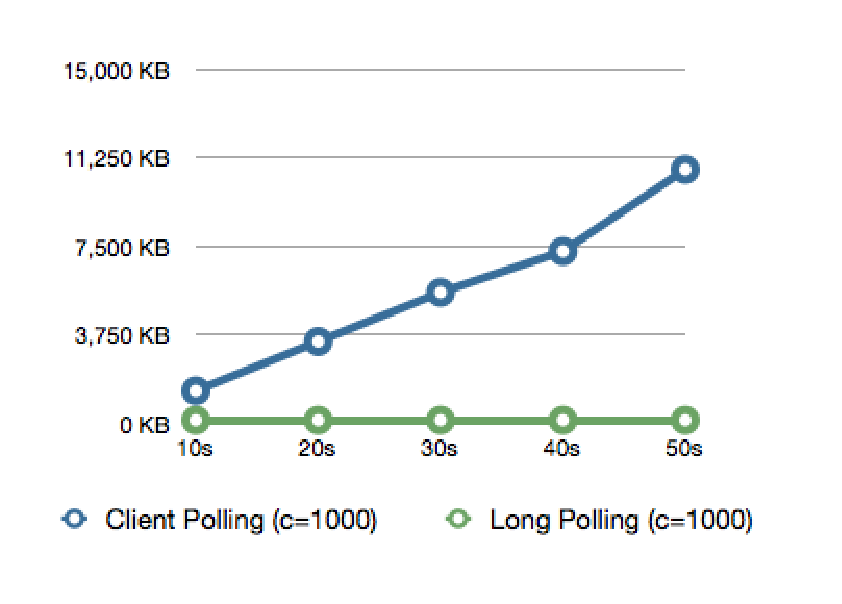
\includegraphics[scale=0.60]{figures/io.eps}
    \caption{Network Traffic of Pull \& Push Models}
    \label{fig:traffic}
\end{figure}


\begin{table}
\centering \caption{\label{tb:mpt_all} Mean Publish Trip Time (second)}
\begin{tabular}{|l|l|l|l|l|l|}
    \hline cc=10 & 10 sec & 20 sec & 30 sec & 40 sec & 50 sec \\
    \hline CP & 0.6 & 0.7 & 0.5 & 0.7 & 0.8 \\
    \hline MLP & 0.1 & 0.0 & 0.1 & 0.2 & 0.1 \\
    \hline ELP & 0.2 & 0.1 & 0.1 & 0.4 & 0.2 \\
    \hline
    \hline cc=100 & 10 sec & 20 sec & 30 sec & 40 sec & 50 sec \\
    \hline CP & 0.8 & 1.1 & 2.5 & 3.1 & 2.7 \\
    \hline MLP & 0.5 & 0.4 & 0.5 & 0.8 & 1.1 \\
    \hline ELP & 0.7 & 0.4 & 0.8 & 1.2 & 0.9 \\
    \hline
    \hline cc=1000& 10 sec & 20 sec & 30 sec & 40 sec & 50 sec \\
    \hline CP & 2.8 & 3.4 & 4.5 & 5.3 & 7.2 \\
    \hline MLP & 2.3 & 2.9 & 2.7 & 3.5 & 3.4 \\
    \hline ELP & 2.4 & 2.8 & 1.8 & 2.4 & 2.9 \\
    \hline
\end{tabular}
\end{table}

\begin{figure}[htb!]
\centering%
    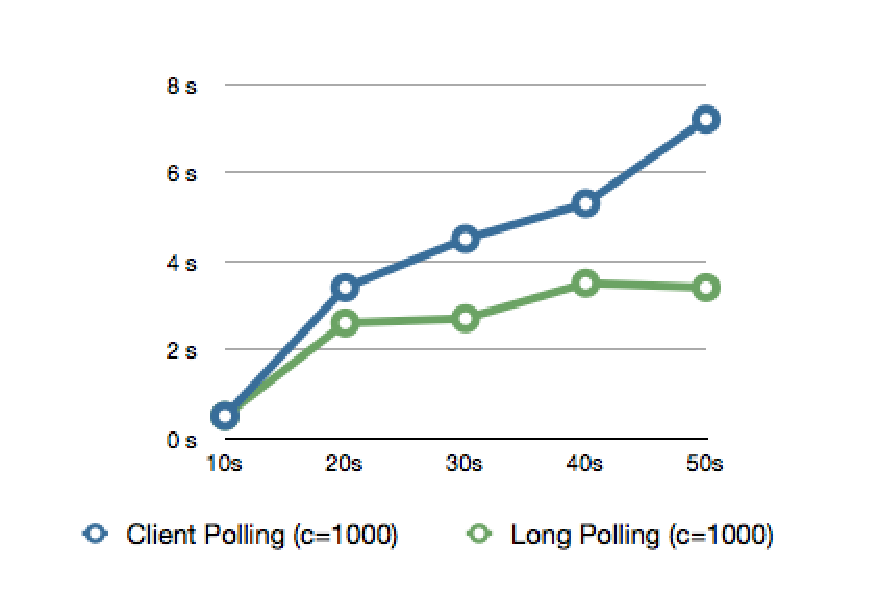
\includegraphics[scale=0.60]{figures/latency.eps}
    \caption{Mean Publish Trip Time of Pull \& Push Models}
    \label{fig:traffic_latency}
\end{figure}

\subsection{Event vs. Thread\\}

Here we compared the performance between event-based long polling model
and the multithreading long polling model. In the following evaluation
we tested the {server memory usage(SMU)}, {\bf mean publish trip time
(MPT)}, {\bf received message percentage(RMP)} with large number of
active connections(from 500-16000).

Figure \ref{fig:et_memory} shows the server memory usage of both models.
The event-based model demonstrates an excellent memory usage as the
number of active connections increases, while the memory usage of 
multithreading model soars rapidly and reaches $100\%$ when the active
connections' number goes to $8000$.

Figure \ref{fig:et_latency} and figure \ref{fig:et_rate}, show the mean
publish trip time and received message percentage. Event-based model 
significantly excels multithreading model in both evaluation.

Thus we claimed multithreading approach is not a good choice as its
memory usage and possible context switch may incur very large overhead,
which heavily lowered the system performance. The event-based mode, on
the other hand, demonstrates a slower performance decrease as the
number of concurrent connections increases.

\begin{figure}[htb!]
\centering%
    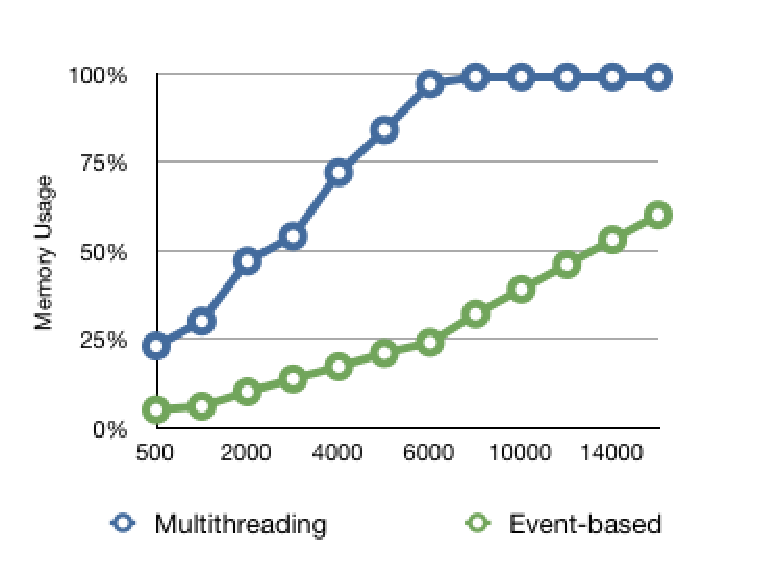
\includegraphics[scale=0.70]{figures/et_memory.eps}
    \caption{Server Memory Usage}
    \label{fig:et_memory}
\end{figure}

\begin{figure}[htb!]
\centering%
    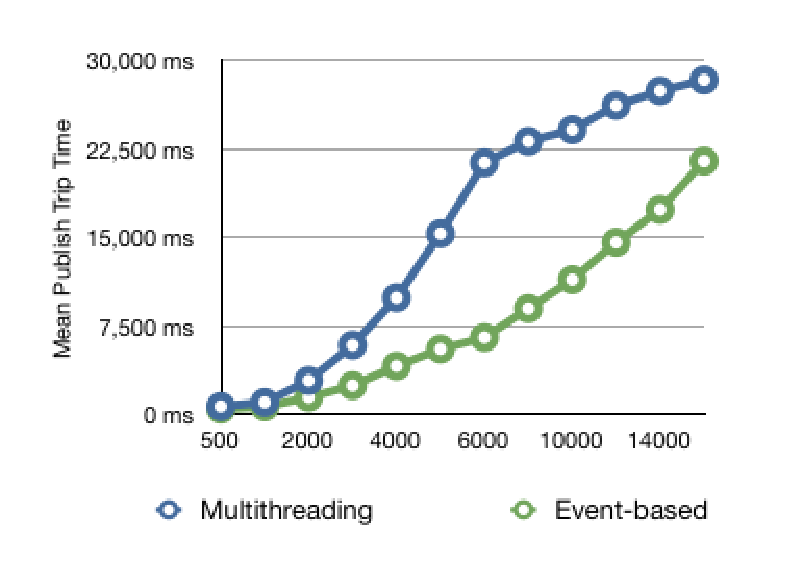
\includegraphics[scale=0.70]{figures/et_latency.eps}
    \caption{Mean Publish Trip Time}
    \label{fig:et_latency}
\end{figure}

\begin{figure}[htb!]
\centering%
    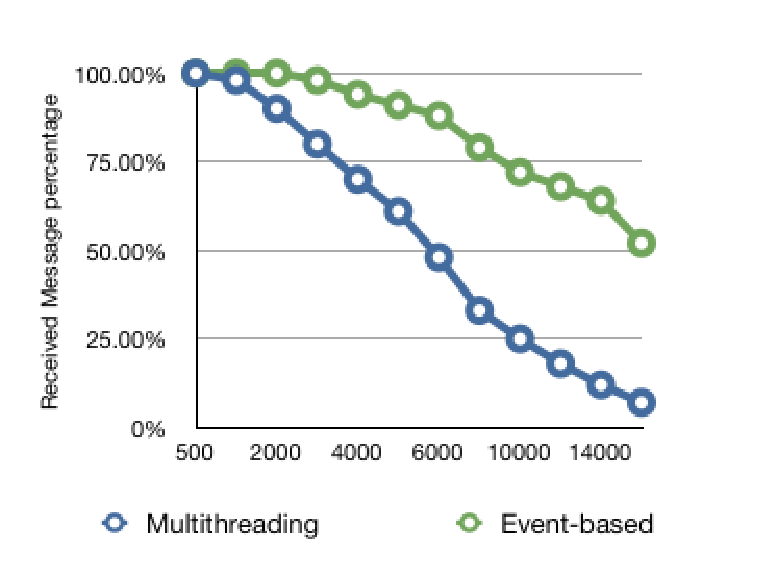
\includegraphics[scale=0.70]{figures/et_rate.eps}
    \caption{Received Message Percentage}
    \label{fig:et_rate}
\end{figure}


\subsection{Extending PushUp Server\\}

* Design goal: Comparison between different models, what are the expected experimental results.

* How do you conduct the experiment?

* What is the exp results?

* Experiment analysis: What can you see from the experiment results? Does it match your expectation?


How they can serve large amount of active connection.

Metrics:

Up to 20000 connections.

HAProxy, very simple load balancing.

1, 2, 3, 4, 5

The Load balance create a little overhead (how much?).

But overall the overhead is acceptable.




\subsection{Measuring the Active Connections\\}


\section{Related Work\\}

\subsection{Event vs. Thread\\}

Some stuff mentioned in the class.

\subsection{Server Push technologies\\}

In \cite{Engin}, Bozdag \emph{et al} provided a complete comparison 
and evaluation of different server push technologies, including the 
HTTP pull, Flash XML socket, Java RMI, etc. As a conclusion the authors 
stated that "an event-driven model on the server side is necessary" 
owing to its , lower consumption of the computing resource, less network
traffic etc.

Another paper \cite{duquennoy09consistency} performs the quantitative 
analysis of the consistency and scalability of several different server
push technologies. As the experimental results showed the event-driven
long polling model shows an excellent efficiency and scalability.



%
% The following two commands are all you need in the
% initial runs of your .tex file to
% produce the bibliography for the citations in your paper.
\bibliographystyle{abbrv}
\bibliography{sigproc}  % sigproc.bib is the name of the Bibliography in this case
% You must have a proper ".bib" file
%  and remember to run:
% latex bibtex latex latex
% to resolve all references
%
% ACM needs 'a single self-contained file'!
%
%APPENDICES are optional
%\balancecolumns
% That's all folks!
\end{document}
